
\chapter{Implementation}
In this chapter, the process of implementation will be covered, starting by the architecture and the tools to the results and how everything fits together.

\section{Tools}
\subsection{Python}
Python\cite{WelcomePythonOrg} is a programming language that can be used in many contexts and is suitable for any type of use thanks to specialized libraries. However, it is particularly used as a scripting language to automate simple but tedious tasks. It is also used as a prototype development language when a functional application is needed before optimizing it with a lower level language. It is particularly widespread in the scientific world, and has many libraries optimized for numerical calculations\cite{PythonLangageWikipedia}.
\paragraph{Pandas:} 

Pandas\cite{PandasPythonData} is a library written for the Python programming language for data manipulation and analysis. In particular, it offers data structures and operations for manipulating numerical arrays and time series. Pandas is free software under the BSD license.


\begin{wrapfigure}[10]{r}{4cm}
	\vspace{-10pt}
	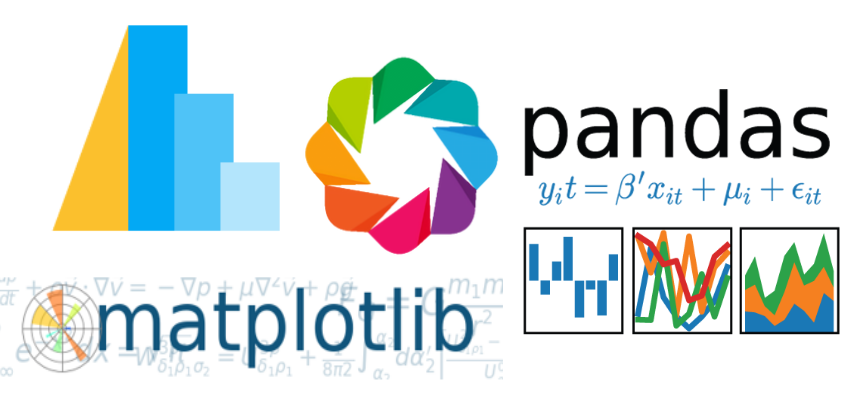
\includegraphics[width=4cm]{images/chapter4/python_pandas.png}
	\vspace{-10pt}
	\caption{{\footnotesize Python et Pandas Logo.}}
\end{wrapfigure}


The main data structures offered by Pandas are series (to store data according to one dimension - size according to an index), DataFrames (to store data according to 2 dimensions - rows and columns), Panels (to represent data according to 3 dimensions, 4D Panels or Data Frames with hierarchical indexes also called Multi Index (to represent data according to more than 3 dimensions - hypercube))\cite{Pandas2020}.



\subsection{Talend}
\label{sec:talend}
We used  Talend Open Studio to create and develop ETL processes. It is a tool based on Java and with an interface derived from that of Eclipse (Figure \ref{fig:Talend}). It allows you to design ETL processes visually, and offers more than nine hundred components (the following list is not exhaustive)\cite{TalendOpenStudio}: 
\begin{itemize}
\renewcommand{\labelitemi}{$\bullet$}
\item Connect to different data sources for reading and writing:
\begin{itemize}
\item Flat files, .xml, .csv, xls, etc.
\item Relational databases (Postgresql, MsSql, etc) and Nosql.
\end{itemize}
\item To manipulate the data, namely:
\begin{itemize}
\item Filter them.
\item Apply aggregate functions on them.
\item Sort them.
\end{itemize}
\item To organize data flows.
\end{itemize}
These components are then assembled as needed to design ETL processes\cite{mehdiPfe}.
\begin{figure}[h!]
    \center
    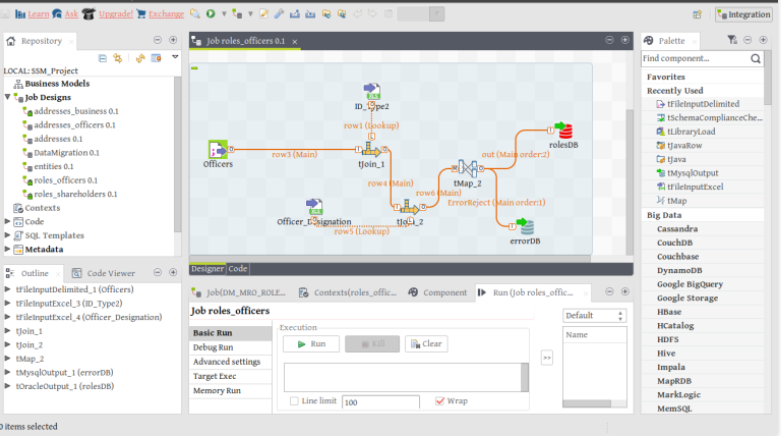
\includegraphics[width=0.75\textwidth]{images/chapter4/talendInterface.png}
    \caption{Talend Interface.}
    \label{fig:Talend}
\end{figure}
\newpage
\subsection{Tableau}
\label{sec:tableau}
Tableau is an excellent data visualization and business intelligence tool used for reporting and analyzing vast volumes of data. It helps users create different charts, graphs, maps, dashboards, and stories for visualizing and analyzing data, to help in making business decisions. Tableau supports powerful data discovery and exploration that enables users to answer important questions in seconds, it can connect to several data sources that other BI tools do not support. Tableau enables users to create reports by joining and blending different datasets and it supports a centralized location to manage all published data sources within an organization\cite{WhatTableauUltimate}.
\begin{figure}[h!]
    \center
    
\includegraphics[width=0.75\textwidth]{images/chapter4/TableauLogo.png}
    \caption{Tableau Logo.}
    \label{fig:tableau}
\end{figure}
\subsection{Highcharts}
Highcharts is a software library for charting written in pure JavaScript meant to enhance web applications by adding interactive charting capability. 
It has all the tools needed to create reliable and secure data visualizations by
providing a wide variety of charts. For example, line charts, spline charts, area charts, bar charts, pie charts and so on.They offer wrappers for the most popular programming languages (.Net, PHP, Python, R, Java) as well as iOS and Android, and frameworks like Angular, Vue, and React\cite{InteractiveJavascriptCharts}.
\begin{figure}[h!]
    \center
    
\includegraphics[width=0.25\textwidth]{images/chapter4/highchart.png}
    \caption{Highcharts Logo.}
    \label{fig:Highcharts}
\end{figure}

\section{Result}
To validate the proposed solution, we visualize the data  using various technologies highlighted in previous sections, in this section we will go through the results that were obtained by this investigatory effort.
\subsection{Processed Data Result}
After the data cleansing using python and its libraries, and the data processing using Talend, we got these results:


\begin{figure}[h!]
    \center
    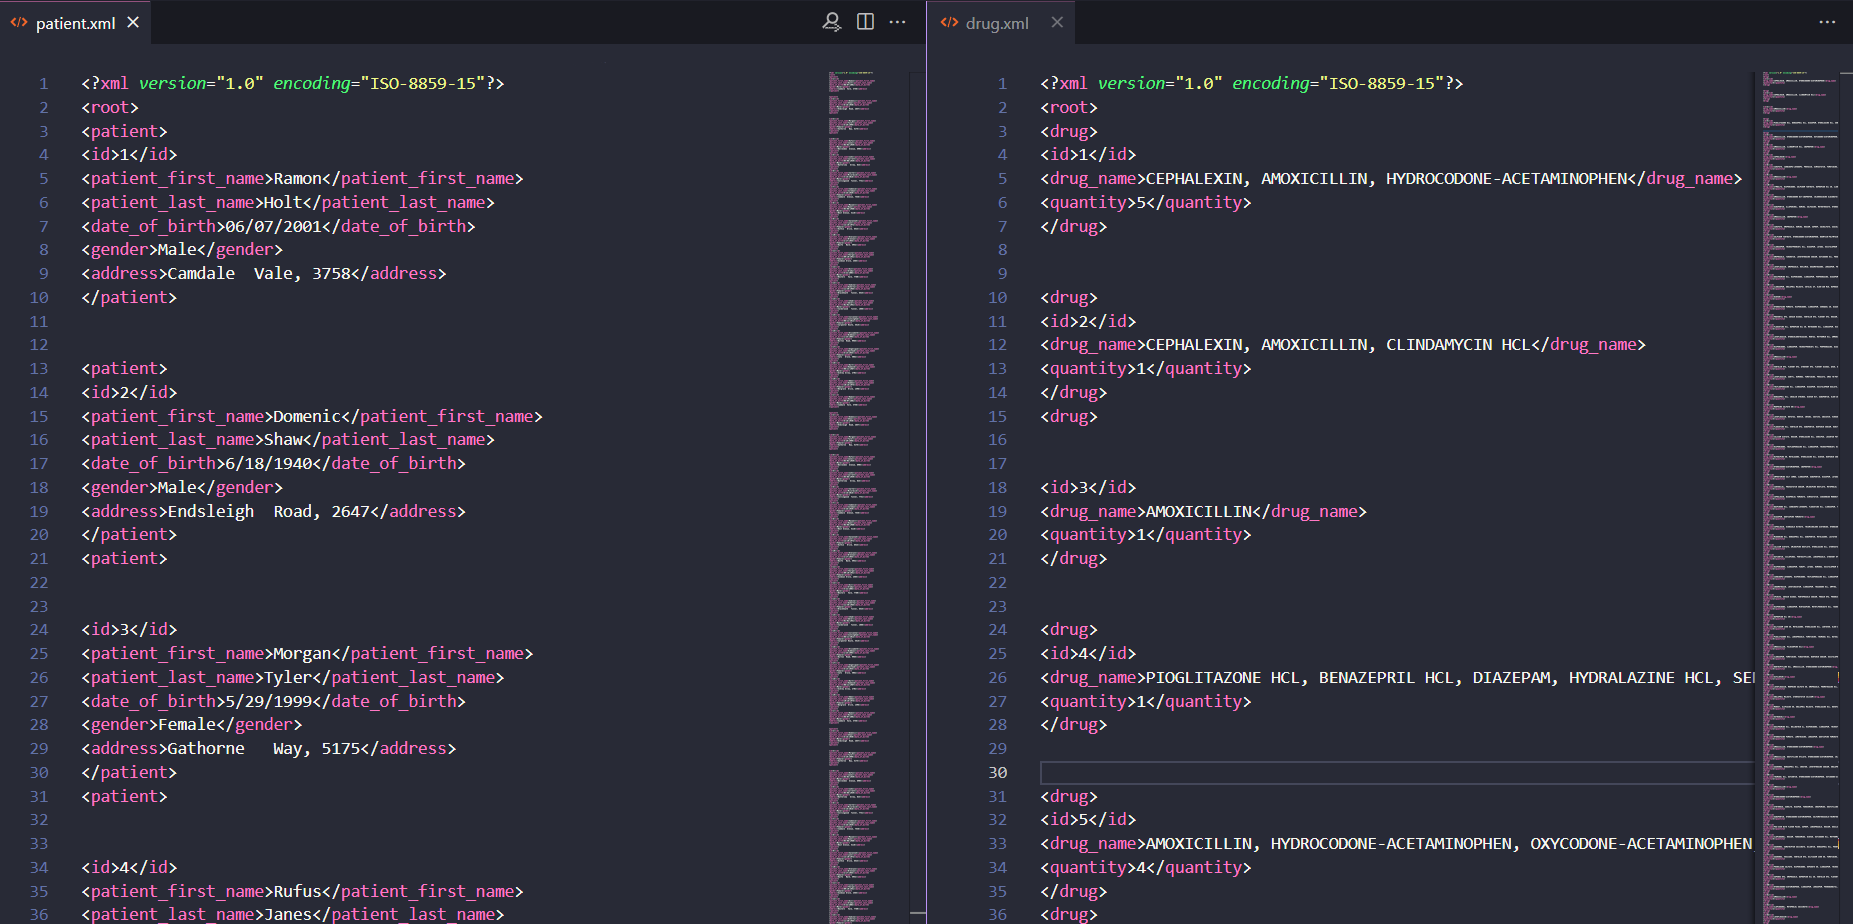
\includegraphics[width=0.90\textwidth]{images/chapter4/result1.PNG}
    \caption{Patient Informations and the related drugs.}
    \label{fig:resultone}
\end{figure}
\begin{figure}[h!]
    \center
    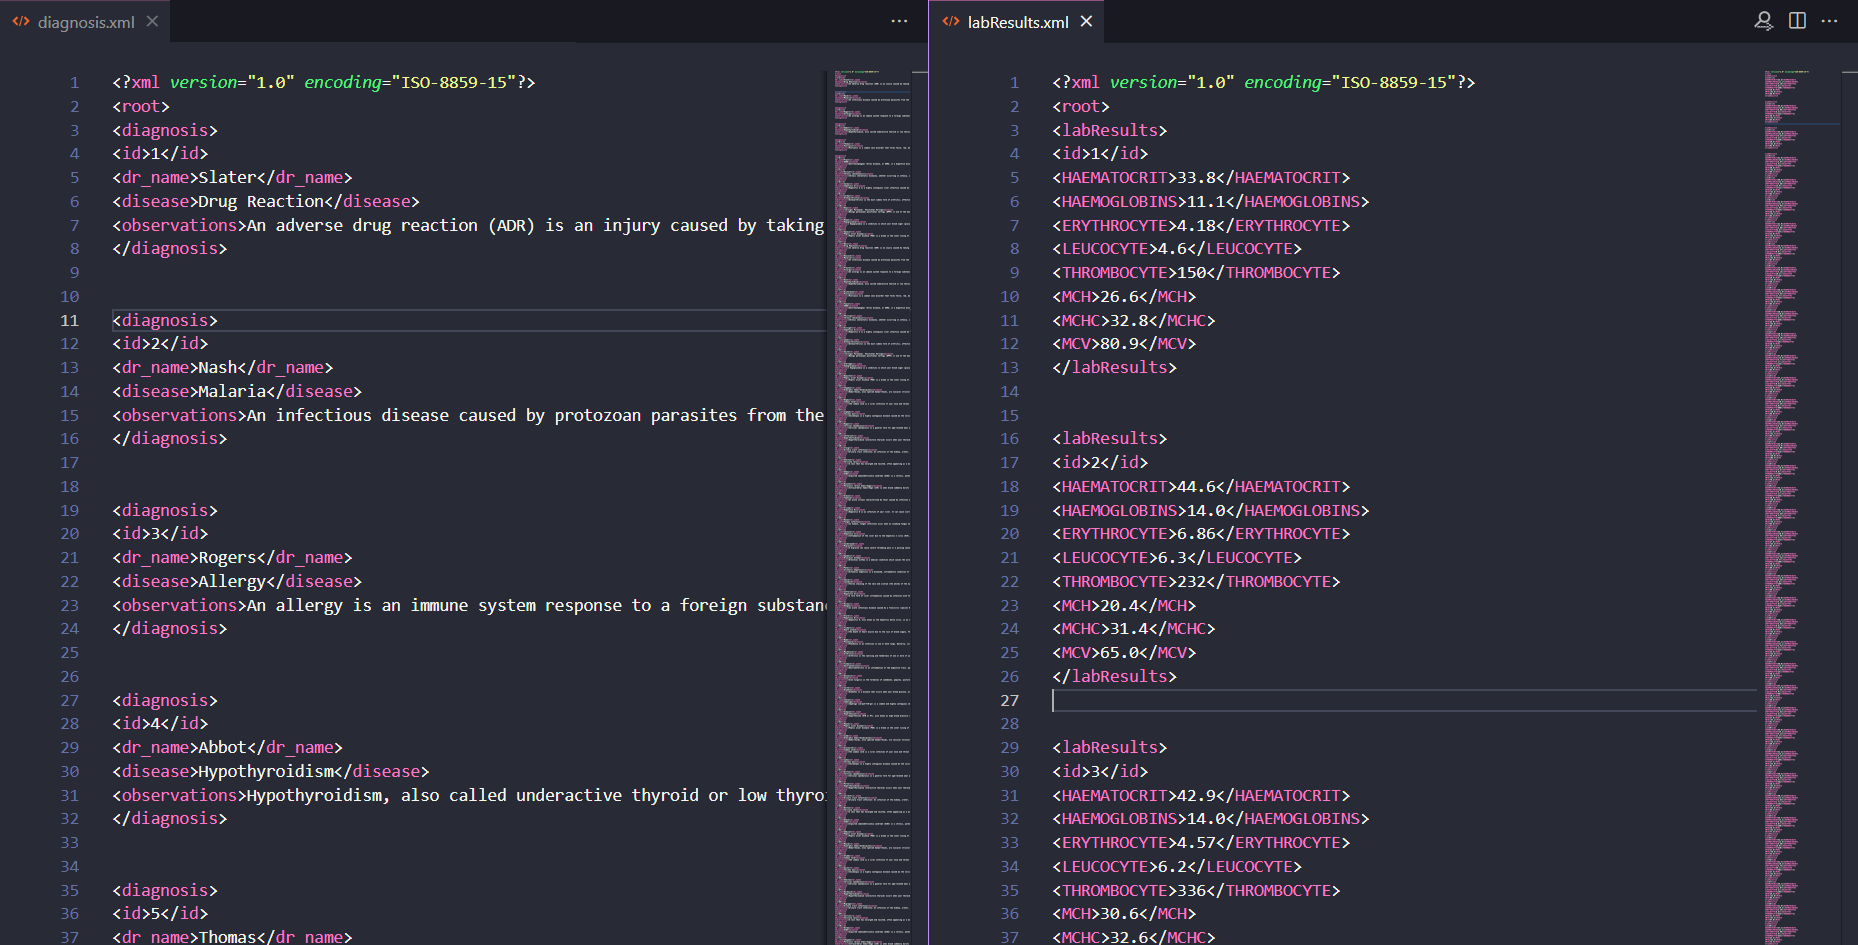
\includegraphics[width=0.90\textwidth]{images/chapter4/result2.PNG}
    \caption{Patient's diagnosis and the his Lab tests results.}
    \label{fig:resulttwo}
\end{figure}

\subsection{Dashboards}
The presented dashboards illustrate some different ways we can visualize some relevant patient data we obtained.\\
Both dashboards are a web application developed using bootstrap\cite{IntroductionBootstrapV5}  framework and the Highcharts  library.

\begin{itemize}
    \renewcommand{\labelitemi}{$\bullet$}
    \item \textbf{Administration Dashboard:}
     \begin{figure}[h!]
        \center
        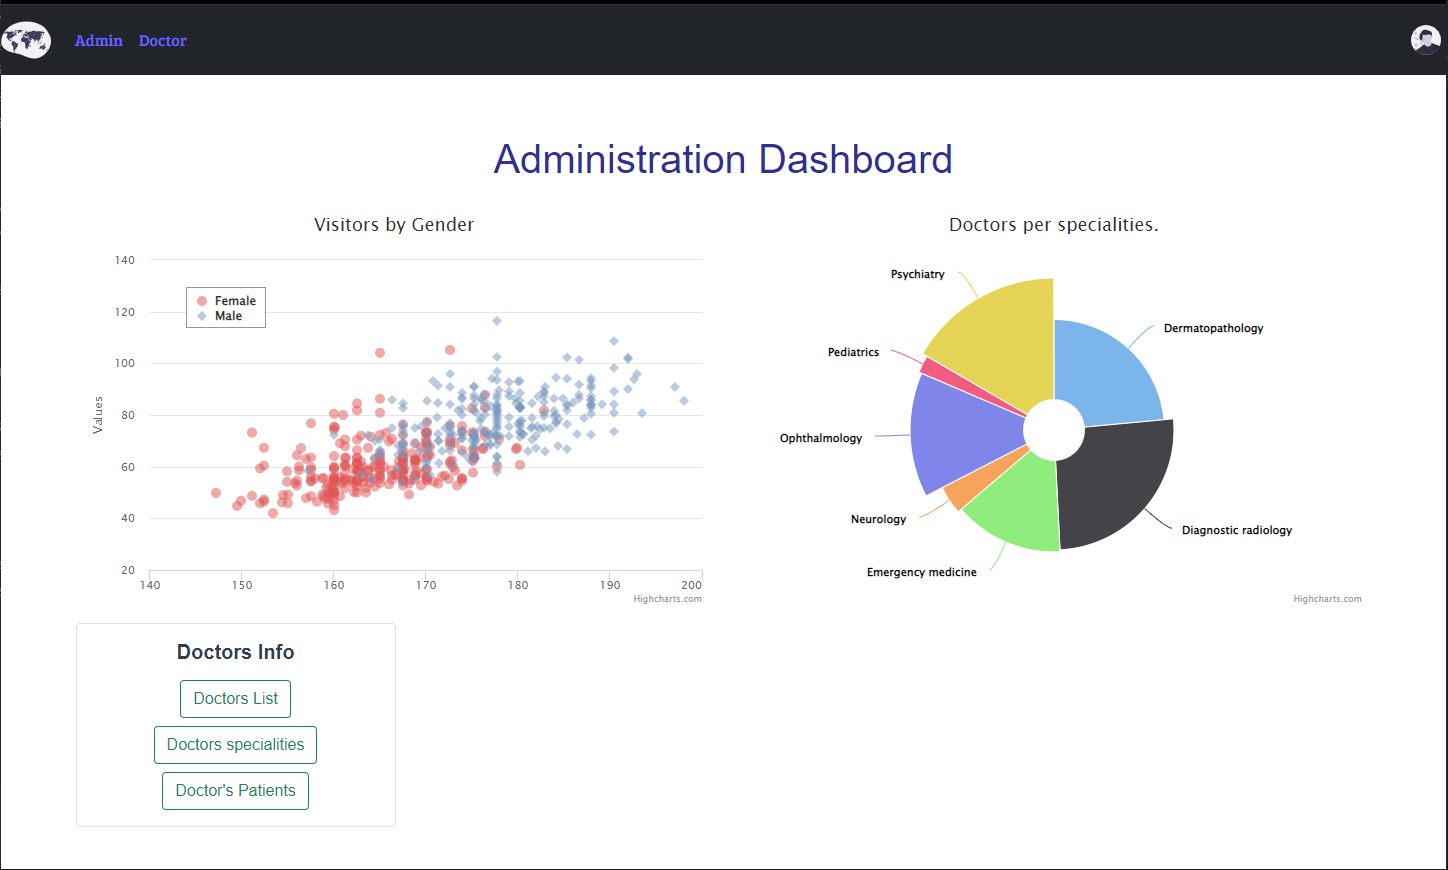
\includegraphics[width=0.90\textwidth]{images/chapter4/adminDashboard.PNG}
        \caption{Administration Dashboard illustrates some of Viz results.}
        \label{fig:admin}
    \end{figure}
    \newpage
    \item \textbf{Doctor Dashboard:}
    \begin{figure}[h!]
        \center
        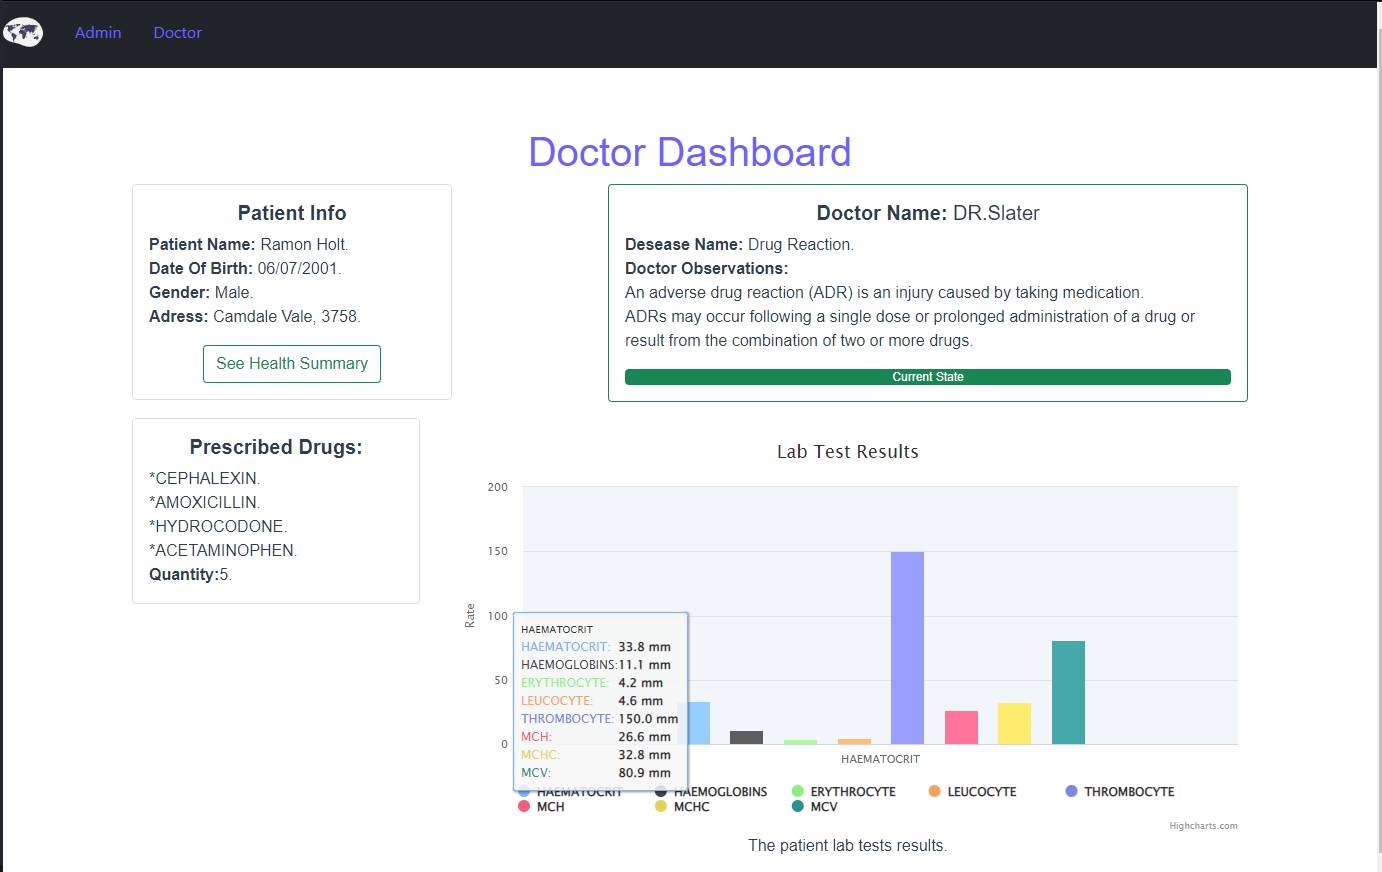
\includegraphics[width=0.90\textwidth]{images/chapter4/doctor.PNG}
        \caption{Doctor Dashboard.}
        \label{fig:doctor}
    \end{figure}
\end{itemize}